\documentclass[a4paper]{article}
% define the title
\usepackage{textcomp}
\usepackage{amsmath}
\newcommand\numberthis{\addtocounter{equation}{1}\tag{\theequation}}
\usepackage{graphicx}
\usepackage{subcaption}
\usepackage[x11names]{xcolor}                     %Additional colors
\usepackage{tikz}
\usepackage{euler}
\author{Nandakishore MM}
\title{Formulation of the variational principle}
\begin{document}
	% generates the title
	\maketitle
	
	\tableofcontents
	
	\newpage


	\section{Introduction}
	The classical problem of steady inviscid subsonic flow past an aerofoil can be formulated in two ways. The usual formulation is as a boundary value problem consisting of a set non linear partial differential equations and a set of boundary conditions. However, it can also be formulated in terms of complementary variational principles. This report describes a variational method for obtaining numerical solutions. The method consists of replacing the infinitely dimensional variational problem by a finitely dimensional problem by means of finite differences, and an approximate maximizing function is then found by standard methods. 

	\section{Formulation}
	
	
	\begin{figure}
		\centering
  		\begin{tikzpicture}
			\draw[thick,<->] (-4.5,0) -- (4.5,0) node[anchor=north west] {x};
			\draw[thick,<->] (0,-4.5) -- (0,4.5) node[anchor=south east] {y};
			\draw[very thick] (0,0) circle(3);
			\draw (2.5,2.5) node {$C$};
			\foreach \y in {-4,-2,...,4}
				\draw[thick, ->] (-7,\y) -- (-5,\y);
			\draw (-6,4.2) node {$U$};
  		\end{tikzpicture}
  		\caption{Sketch of the flow field}
  	\end{figure}	
  	
	The boundary value problem for plane subsonic flow	 past an aerofoil can be formulated as follows.
	
	Let $\vec{u}=(u_1,u_2)$ be the velocity vector in the Cartesian coordinate system. Far from the aerofoil, C $\vec{u}=(U,0)$ where $U$ is a constant.
	
	For an irrotational flow, a velocity potential can be defined as 
	$$ \vec{u} = \nabla \phi$$
	
	The pressure and density are defined by $p$ and $\rho$ respectively. The speed of sound is defined by
	$$c^2=\frac{dp}{d\rho}$$
	
	$$p=p_0 \Biggl(
	1-\frac{q^2}{2\beta c^2_0}
	\Biggr)^\alpha$$

	$$\rho=\rho_0 \Biggl(
	1-\frac{q^2}{2\beta c^2_0}
	\Biggr)^\beta$$	
	
	where
	
	$$q^2 = \vec{u}.\vec{u}, \qquad \alpha=\frac{\gamma}{\gamma-1},
	\qquad \beta=\frac{1}{\gamma-1}$$
	
	the suffix $0$ indicates stagnation values.
	
	The boundary value problem for $\phi$ is equivalent to a variational problem of maximizing the integral 
	\begin{equation} \label{var_eq}
		 J[\phi] = \int_{R_1} pdV + \int_B\phi h dA
	\end{equation}
	($dV = $ area element, $dA = $ arc length element of $B=C$). Then $J[\phi]$ is a maximum if $\nabla.(\rho \vec{u} = 0$ and
	$\rho\vec{u}.\hat{n} = h$ on $B$. Here the normal mass flu $h$ is prescribes on $B$ such that 
	$$ \text{outflow} = \int_B hdA = 0$$
	
	If the flow region $R_1$ becomes infinite, the variational integral (\ref{var_eq}) becomes unbounded. To remove this difficulty, the integral can be formulated as follows
	\begin{equation} \label{var_eq2}
		J[\phi] = \int\int_\infty [ p-p_\infty+p_\infty.\nabla(\phi-\phi_\infty) ]dxdy
	\end{equation}
	
	where 
	
	$\qquad p_\infty = $ pressure at infinity, 
	
	$\qquad \rho_\infty = $ density at infinity, 
	
	$\qquad \phi_\infty = $ potential for a uniform stream 
	
	$\qquad \phi_0 = $ potential for incompressible flow past $C$.
	
	To extend the method to a general class of aerofoils, a conformal mapping from the aerofoil $C$ onto a unit circle can be used. Let $z=x+iy$ and $\sigma=r(\cos \theta + i \sin \theta)$, then,, the transform modulus is given by	
	$$
	T = \Biggl|\frac{dz}{d\sigma}\Biggr|
	= (x_r^2+y_r^2)^\frac{1}{2}
	$$
	The Jacobian of the transformation is
	$$
	J= \frac{\partial(x,y)}{\partial(r,\theta)}
	= x_r y_\theta - x_\theta y_r
	$$
	
	Since the transformation is conformal
	$$
	y_\theta = rx_r \qquad \text{and} \qquad y_r=-\frac{1}{r}x_\theta
	$$
	so
	$$
	T^2 = x_r^2 + \frac{1}{r^2}x_theta^2
	$$
	and
	$$
	J=r\Biggl(
	x^2_r+\frac{1}{r^2}x^2_\theta
	\Biggr)
	$$
	Hence 
	\begin{equation} \label{J}
		 J=rT^2
	\end{equation}
	
	The coordinates $r, \theta$ are orthogonal so the element of length $ds = |dz|$ is given by
	$$
	ds^2 = h_1^2dr^2 + h_2^2d\theta^2
	$$
	Also
	$$
	ds^2 = |dz|^2 = \Biggl|\frac{dz}{d\sigma}\Biggr|^2|d\sigma|^2
	$$
	$$=T^2(dr^2+r^2d\theta^2)$$
	
	Therefore
	$$h1=T \qquad \text{and} \qquad h_2=rT$$	
	so
	$$ \nabla \phi = \frac{1}{T} 
	\Biggl(
		\hat{r}\phi_r + \frac{\hat{\theta}}{r}\phi_\theta
	\Biggr)
	$$
	Since
	$$q^2=(\nabla \phi)^2$$
	and
	$$\phi = U(r\cos \theta+\chi)$$
	we have
	\begin{equation}\label{q2}
		q^2 = 
		\frac{U^2}{T^2}
		\Biggl[
			1 + 2\cos\theta. \chi_r - \frac{2}{r} \sin\theta. \chi_\theta +
			\chi_r^2 + \frac{1}{r^2}\chi_\theta^2
		\Biggr]
	\end{equation}
	Also
	$$
	p = p_0\Biggl(
		1 - \frac{q^2}{2\beta c_0^2}
	\Biggr)^\alpha
	$$
	and by using the relation
	$$
	p_0 = \Biggl(\frac{\rho_0}{\rho_\infty}\Biggr)^\gamma p_\infty
	$$
	we get after some manipulation
	\begin{equation} \label{p}
	p = p_\infty \Biggl[
		1+\frac{(\gamma-1)M_\infty^2}{2T^2}
		\Biggl(
			T^2-1-2\cos\theta.\chi_r +
			\frac{2}{r}\sin\theta.\chi_\theta
			-\chi_r^2-\frac{1}{r^2}\chi_\theta^2
		\Biggr)
	\Biggr]^\alpha
	\end{equation}
	where the free stream Mach number $M_\infty$ is defined by
	$$
	M^2_\infty = \frac{2\beta U^2}{2\beta c_0^2-U^2}
	$$
	Now
	$$
	\frac{\gamma p_\infty}{\rho_\infty} = c_0^2 - \frac{U^2}{2\beta}
	$$
	Thus since
	$$\phi_o = U\Biggl(r+\frac{1}{r}\Biggr)\cos\theta ,$$
	\begin{equation}	\label{rho_del_phi}
		\rho_\infty \nabla\phi_0 . \nabla(\phi-\phi_\infty) = 
		p_\infty \frac{\gamma M^2_\infty}{T^2}
		\Biggl[
			\frac{r^2-1}{r^2}\cos_theta.\chi_r
			-\frac{r^2-1}{r^3}\sin \theta.\chi_\theta
		\Biggr]
	\end{equation}		
	
	When the expressions (\ref{J}), (\ref{p}) and (\ref{rho_del_phi}) are used in (\ref{var_eq2}), the variational integral becomes
	\begin{equation} \label{var_int}
	\begin{split}		
		J[\chi] = p_\infty \int_0^{2\pi} \int_1^\infty
		\Biggl\{
			\Biggl[
				1 + \frac{(\gamma-1)M_\infty^2}{2T^2}
				\Biggl(
					T^2-1-2\cos\theta.\chi_r+\frac{2}{r}\sin\theta.\chi_\theta - \chi_r^2-\frac{1}{r^2}\chi_\theta^2
				\Biggr)
			\Biggr]^\alpha \\
			-1+\frac{\gamma M_\infty^2}{T^2}
			\Biggl(
				\frac{r^2-1}{r^2}\cos\theta.\chi_r
				- \frac{r^2+1}{r^3}\sin\theta.\chi_\theta
			\Biggr)
		\Biggr\}rT^2dr
	\end{split}
	\end{equation}
	The boundary conditions on $\chi$ are
	\begin{equation}\label{bc}
	\begin{split}
		\frac{\partial\chi}{\partial r} = -\cos\theta \qquad \text{at} \qquad r=1, \\
		\chi = 0 \left(\frac{1}{r}\right) \qquad \text{as} \qquad r \rightarrow \infty
	\end{split}
	\end{equation}
	
	The local Mach number$M$ and the local non dimensional pressure $p_L$ are given by
	\begin{equation}\label{mach}
		M = M_\infty\frac{q}{U}
		\Biggl[
			1 + \frac{1}{2}(\gamma-1)M_\infty^2
			\left(1-\left(\frac{q}{U}\right)^2\right)
		\Biggr]	^\frac{1}{2}
	\end{equation}
	\begin{equation}\label{pressure}
		p_L = \frac{p}{p_\infty} = 
		\Biggl[
			1 + \frac{1}{2}(\gamma-1)M_\infty^2
			\left(1-\left(\frac{q}{U}\right)^2\right)		
		\Biggr]^\frac{\gamma}{\gamma-1}
	\end{equation}
	where q is given by equation (\ref{q2})
	
	The transform modulus for an ellipse is given by
	\begin{equation}\label{T}
		T^2 = \frac{1}{r^4} \left[
			\left(r^2+\lambda^2\right)^2 - 
			4\lambda^2r^2\cos^2\theta
		\right]
	\end{equation}		
	where $\lambda^2$ is the following function of $\tau$, the thickness ratio of the ellipse,
	\begin{equation}
		\lambda^2 = \frac{1-\tau}{1+\tau}
	\end{equation}
	
  	\section{Numerical Method}
	
	The objective of the calculation is to find for given $M_\infty$ and aerofoil shape a function $\chi$ which maximizes $J[\chi]$ as given by (\ref{var_int}) subject to boundary conditions (\ref{bc}).
	
	
	\subsection{Domain}
	For non lifting symmetric bodies (about $y=0$), it is only necessary to treat the interval $0 \leq \theta  \leq \pi$.
	
	Since the derivatives in both directions are approximated by finite differences, it is necessary to have a finite computation region. This is obtained by replacing the infinite integration limit on $r$ by a finite limit $R$ and insisting that the reduced potential $\chi$ satisfies an appropriate condition at $r=R$. The simplest condition to impose is that $\chi$ equals the reduced potential for incompressible flow at $r=R$. 
	
	Thus the variational integral reduces to
	\begin{equation}\label{var_int_reduced}
	J[\chi] = p_\infty \int^\pi_0 \int^R_1 F(r,\theta,\chi_r,\chi_\theta)dr
	\end{equation}
	where
	$$
	F = \Biggl\{
			\Biggl[
				1 + \frac{(\gamma-1)M_\infty^2}{2T^2}
				\Biggl(
					T^2-1-2\cos\theta.\chi_r+\frac{2}{r}\sin\theta.\chi_\theta - \chi_r^2-\frac{1}{r^2}\chi_\theta^2
				\Biggr)
			\Biggr]^\alpha
			$$
			$$
			-1+\frac{\gamma M_\infty^2}{T^2}
			\Biggl(
				\frac{r^2-1}{r^2}\cos\theta.\chi_r
				- \frac{r^2+1}{r^3}\sin\theta.\chi_\theta
			\Biggr)
		\Biggr\}rT^2
	$$
	
	The boundary conditions are now
	\begin{align*}
	\frac{\partial\chi}{\partial\theta}&=0 &\text{at} \qquad  &\theta=0,\pi \\
	\frac{\partial\chi}{\partial r}&=-\cos \theta &\text{at} \qquad  &r=1 \\	
	\chi &=\frac{1}{R}\cos \theta &\text{at} \qquad  &r=R \numberthis \label{bcs}
	\end{align*}

	\subsection{Discretisation}
	
	$$r = 1,\ldots,R; \qquad  k_j = r_{j+1} - r_j $$
	$$\theta = 0,\ldots,\pi; \qquad h_i = \theta_{i+1} - \theta_i  $$	
	
	$\theta$ varies linearly from $0$ to $\pi$. $r$ is mapped as $r=1/\sigma$, where $\sigma$ varies linearly in the range [1/R, 1]. 	
	
	Thus, the infinitely dimensional variational problem is now replaced by a finite-dimensional problem. Consider four neighbouring points as shown in figure (\ref{grid}). The derivatives of $\chi$ in the rectangle $(i,j)$ can be approximated as
	$$
	\frac{\partial \chi}{\partial \theta} = 
	\frac{\chi_{i+1,j}+\chi_{i+1,j+1}-\chi_{i,j}-\chi{i,j+1}}{2h_i}
	$$
	$$
	\frac{\partial \chi}{\partial \theta} = 
	\frac{\chi_{i,j+1}+\chi_{i+1,j+1}-\chi_{i,j}-\chi{i+1,j}}{2k_j}
	$$
	
	
	
	
	
	\begin{figure}
		\centering
  		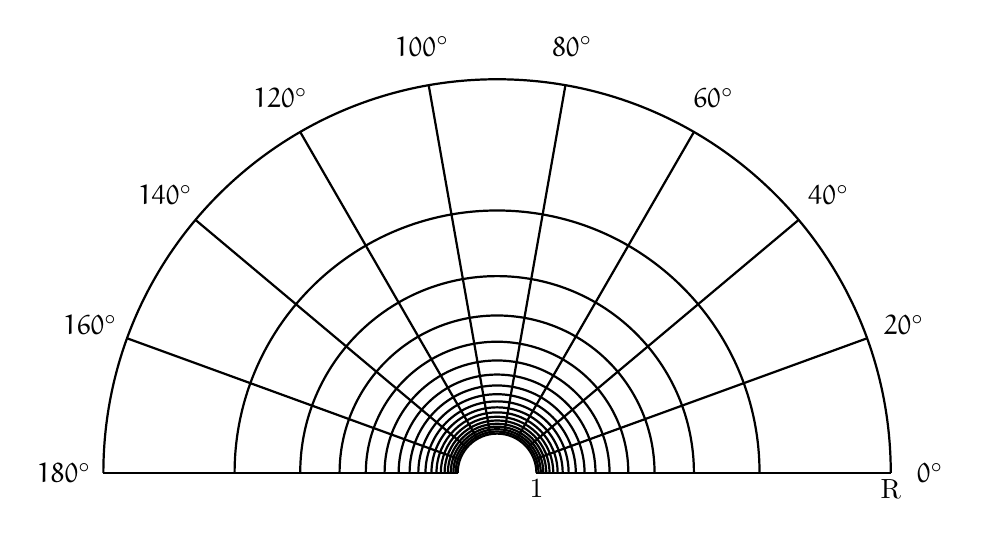
\begin{tikzpicture}
    			%Circles     
    			\foreach \r in {1, 1.05263, 1.11111, 1.17647, 1.25, 1.33333, 1.42857, 1.53846, 1.66667, 1.81818, 2, 2.22222, 2.5, 2.85714, 3.33333, 4, 5, 6.66667, 10}
      			\draw[thick] ({\r / 2},0) arc (0:180:{\r / 2});
    
    			%Rays
    			\foreach \a in {0, 20,...,180}
      			\draw[thick] (\a:.5) -- (\a:5);
   
     		\draw (.5,-.2) node {1};
     		\draw (5,-.2) node {R};
      
    			%Angle labels  
    			\foreach \a in {0, 20,...,180}
      			\draw (\a: 5.5) node {$\a^\circ$};
  		\end{tikzpicture}
  		\caption{Mesh around the body}
	\end{figure}		
	
	\begin{figure}
		\centering
  		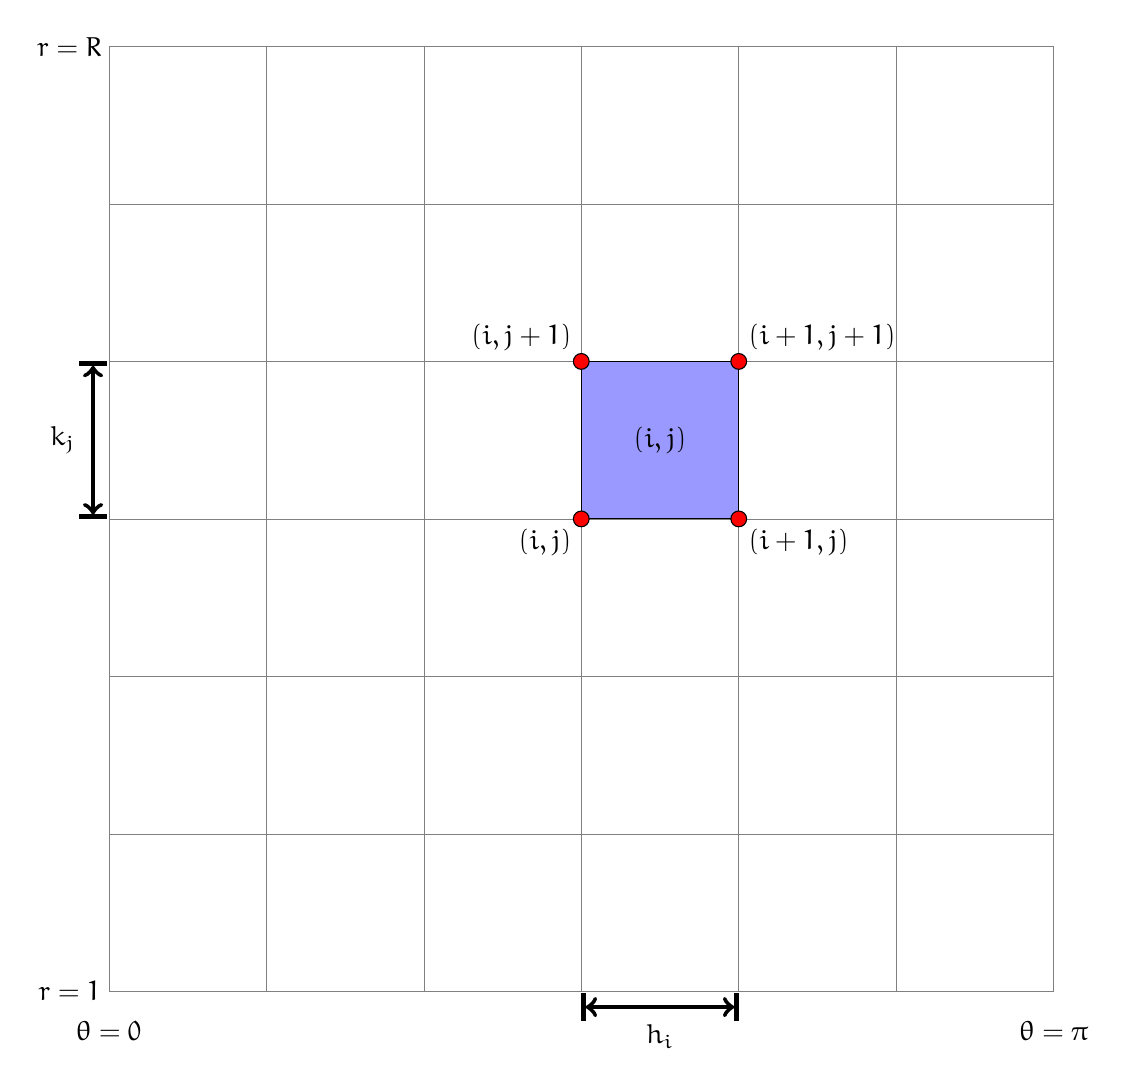
\begin{tikzpicture}
    			\draw[step=2,gray,very thin] (-6,-6) grid (6,6);
    			\filldraw[fill=blue!40!white, draw=black] (0,0) rectangle (2,2);
				\node[anchor=north east] (one) at (0,0) {$(i,j)$};
				\node[anchor=south east] (one) at (0,2) {$(i,j+1)$};
				\node[anchor=north west] (one) at (2,0) {$(i+1,j)$};
				\node[anchor=south west] (one) at (2,2) {$(i+1,j+1)$};
				\node (one) at (1,1) {$(i,j)$};

				\draw[fill=red] (0,0) circle(.1);
				\draw[fill=red] (2,0) circle(.1);
				\draw[fill=red] (0,2) circle(.1);
				\draw[fill=red] (2,2) circle(.1);

				\node (q) at (-6.5,-6) {$r=1$};
				\node (q) at (-6.5,6) {$r=R$};
				\node (q) at (-6,-6.5) {$\theta=0$};
				\node (q) at (6,-6.5) {$\theta=\pi$};

				\draw[|<->|, ultra thick] (0,-6.2) -- (2,-6.2);
				\node[anchor=north] (q) at (1,-6.3) {$h_i$};

				\draw[|<->|, ultra thick] (-6.2,0) -- (-6.2,2);
				\node[anchor=east] (q) at (-6.3,1) {$k_j$};
  		\end{tikzpicture}
  		\caption{Computational domain}
  		 \label{grid}
	\end{figure}	
	
	
	
	For a rectangular region $i,j$, $J[\chi]$ can be approximated as
	\begin{multline}
	J_{i,j} = p_\infty 
	\Biggl\{
		\Biggl[
			1 + \frac{(\gamma-1)M_\infty^2}{2T_{i,j}^2}
			\Biggl(
				T^2 - 1
				- 2\cos\theta '_i \frac{ \chi_{i,j+1} + \chi_{i+1,j+1} - \chi_{i,j} - \chi_{i+1,j}}{2k_j} \\
				+ \frac{2}{r'_j} \sin \theta '_i \frac{ \chi_{i+1,j} + \chi_{i+1,j+1} - \chi_{i,j} - \chi_{i,j+1}}{2h_i} \\
				- \left(
					\frac{ \chi_{i,j+1} + \chi_{i+1,j+1} - \chi_{i,j} - \chi_{i+1,j}}{2k_j}
				\right)^2 \\
				- \frac{1}{r^2}
				\left(
					\frac{ \chi_{i+1,j} + \chi_{i+1,j+1} - \chi_{i,j} - \chi_{i,j+1}}{2h_i}
				\right)^2
			\Biggr)
		\Biggr]^\alpha \\
		- 1 + \frac{\gamma M_\infty^2}{T_{i,j}^2}
		\Biggl(
			\left(
				\frac{r'^2_j-1}{r'^2_j}
			\right)
			\cos \theta '_i \frac{ \chi_{i,j+1} + \chi_{i+1,j+1} - \chi_{i,j} - \chi_{i+1,j}}{2k_j} \\
			- \left(
				\frac{r'^2_j-1}{r'^3_j}
			\right)
			\sin \theta '_i \frac{ \chi_{i+1,j} + \chi_{i+1,j+1} - \chi_{i,j} - \chi_{i,j+1}}{2h_i}
		\Biggr)
	 \Biggr\}
	\end{multline}
	$$	\theta '_i = \theta_i + 0.5h_i; \qquad r '_j = r_j + 0.5 k_j $$
	
	$$	
	T_{i,j}^2 = \frac{1}{r'^4_j}
	\left[
		(r'^2_j+\lambda^2)^2 - 4\lambda^2r'^2_j \cos^2 \theta '_i
	\right]	
	$$
	$$
	\lambda^2 = \frac{1-\tau}{1+\tau}
	$$
	Boundary conditions for $\chi$-
	\begin{enumerate}
	
	\item
	$$
	\frac{\partial \chi}{\partial r} = - \cos \theta; \text{ at } r=1
	$$
	\begin{equation}
	\chi_{i,1}=\frac{1}{k_2+2k_1}
	\left[
		\frac{1}{k_2}
		((k_1+k_2)^2\chi_{1,2} - k_1^2 \chi_{i,3})
		+ k_1(k_1+k_2)\cos \theta
	\right]
	\end{equation}
	
	\item $$ \frac{\partial \chi}{\partial \theta} = 0 \text{ at } \theta = 0, \pi $$
	\begin{equation}
	\chi_{m+1,j} = \chi_{m-1,j} \qquad 
	\chi_{0,j} = \chi_{2,j}
	\end{equation}
	
	\item $$ \chi = \frac{1}{R} \cos \theta \text{ as } r \rightarrow \infty $$
	\begin{equation}
	\chi_{i,n} = \frac{1}{R} \cos \theta_i
	\end{equation}
	
	\end{enumerate}
	
	Summing the contributions for each rectangle, $J[\chi]$ can be approximated as 
	\begin{equation}
	J[\chi] = \bar{J} = 
	\sum\limits_{i=1}^{n-1} \sum\limits_{j=1}^{m-1} J_{i,j}
	\end{equation}
	Therefore, the values of $\chi_{i,j}$ which maximizes this expression is given by the solutions of the equations
	\begin{equation}
	\frac{\partial \bar{J}}{\partial \chi_{i,j}} = 0
	\end{equation}
	$$ i = 1,\ldots,n $$
	$$ j = 2,\ldots,m-1 $$
	
	for a given $i,j$, the equation to maximize can be written in the form (by summing the contributions from the four surrounding rectangles)
	\begin{equation}
	\begin{split}
	g(\chi_{i,j}) = \frac{\partial \bar{J}}{\partial \chi_{i,j}} 
	\sum\limits_{s=(i,j),(i-1,j),(i,j-1),(i-1,j-1)}
	\Biggl[
		\alpha
		\left(
			A_s\chi^2_{i,j} + B_s\chi{i,j} + C_s
		\right)^{\alpha-1}
		\left(
			2A_s\chi_{i,j} + B_s
		\right) \\
		 + D_s
	\Biggr]H_s	
	= 0
	\end{split}
	\end{equation}
	
	Using Newton Raphson method, an improved estimate is given by
	\begin{equation}
	\chi^{(q+1)}_{i,j} = \chi^{(q)}_{i,j}
	- \frac{g(\chi^{(q)}_{i,j})}{g'(\chi^{(q)}_{i,j})}
	\end{equation}
	
	\begin{equation}
	g' = \frac{\partial g_{i,j}}{\partial \chi_{i,j}}
	\end{equation}
	
	
	\subsection{Coefficients A, B, C, D, H}
	The coefficients A, B, C, D, H are given by - 
	
	\begin{align}
		\begin{split}		
		A_{i,j} = -\frac{(\gamma-1)M_\infty^2}{2T_{i,j}^2}
		\left(
			\frac{1}{4k_j^2} + \frac{1}{4{r'}_j^2 h_i}
		\right) \\
		A_{i,j-1} = -\frac{(\gamma-1)M_\infty^2}{2T_{1,j-1}^2}
		\left(
			\frac{1}{4k_{j-1}^2} + \frac{1}{4{r'}_{j-1}^2 h_i}
		\right) \\
		A_{i-1,j} = -\frac{(\gamma-1)M_\infty^2}{2T_{i-1,j}^2}
		\left(
			\frac{1}{4k_j^2} + \frac{1}{4{r'}_j^2 h_{i-1}}
		\right) \\
		A_{i-1,j-1} = -\frac{(\gamma-1)M_\infty^2}{2T_{i-1,j-1}^2}
		\left(
			\frac{1}{4k_{j-1}^2} + \frac{1}{4{r'}_{j-1}^2 h_{i-1}}
		\right)
		\end{split}
	\end{align}
	
	\begin{equation}
		\begin{split}
		B_{i,j} = \frac{(\gamma-1)M_\infty^2}{2T_{i,j}^2}
		\Biggl(
			2\cos \theta '_i \frac{1}{2k_j}
			- \frac{2}{r'_j} \sin\theta '_i \frac{1}{2h_i} \\
			+ \frac{1}{2k_j^2}( \chi_{i,j+1} + \chi_{i+1,j+1} - \chi_{i+1,j} ) \\
			+ \frac{1}{2r'^2_jh_i^2}( \chi_{i+1,j} + \chi_{i+1,j+1} - \chi_{i,j+1} )
		\Biggr) \\
		B_{i,j-1} = \frac{(\gamma-1)M_\infty^2}{2T_{i,j-1}^2}
		\Biggl(
			- 2\cos \theta '_i \frac{1}{2k_{j-1}}
			- \frac{2}{r'_{j-1}} \sin\theta '_i \frac{1}{2h_i} \\
			- \frac{1}{2k_{j-1}^2}( \chi_{i+1,j} - \chi_{i,j-1} - \chi_{i+1,j-1} ) \\
			+ \frac{1}{2r'^2_{j-1}h_i^2}( \chi_{i+1,j-1} + \chi_{i+1,j} - \chi_{i,j-1} )
		\Biggr) \\
		B_{i-1,j} = \frac{(\gamma-1)M_\infty^2}{2T_{i-1,j}^2}
		\Biggl(
			2\cos \theta '_{i-1} \frac{1}{2k_j}
			+ \frac{2}{r'_j} \sin\theta '_{i-1} \frac{1}{2h_{i-1}} \\
			+ \frac{1}{2k_j^2}( \chi_{i-1,j+1} + \chi_{i,j+1} - \chi_{i-1,j} ) \\
			- \frac{1}{2r'^2_jh_{i-1}^2}( \chi_{i,j+1} - \chi_{i-1,j+1} - \chi_{i-1,j+1} )
		\Biggr) \\
		B_{i-1,j-1} = \frac{(\gamma-1)M_\infty^2}{2T_{i-1,j-1}^2}
		\Biggl(
			- 2\cos \theta '_{i-1} \frac{1}{2k_{j-1}}
			+ \frac{2}{r'_{j-1}} \sin\theta '_{i-1} \frac{1}{2h_{i-1}} \\
			- \frac{1}{2k_{j-1}^2}( \chi_{i-1,j} - \chi_{i-1,j-1} - \chi_{i,j-1} ) \\
			- \frac{1}{2r'^2_{j-1}h_{i-1}^2}( \chi_{i,j-1} - \chi_{i-1,j-1} - \chi_{i-1,j} )
		\Biggr) \\
		\end{split}
	\end{equation}
	
	\begin{equation}
		\begin{split}
		C_{i,j} = 1 + \frac{(\gamma-1)M_\infty^2}{2T_{i,j}^2}
		\Biggl(
			T_{i,j}^2 - 1
			- \frac{\cos \theta '_i}{k_j}( \chi_{i,j+1} + \chi_{i+1,j+1} - \chi_{i+1,j} ) \\
			+ \frac{\sin \theta '_i}{r'_j h_i}( \chi_{i+1,j} + \chi_{i+1,j+1} - \chi_{i,j+1} ) \\
			- \frac{1}{4k_j^2}( \chi_{i,j+1} + \chi_{i+1,j+1} - \chi_{i+1,j} )^2 \\
			- \frac{1}{4r'^2_j h_i^2}( \chi_{i+1,j} + \chi_{i+1,j+1} - \chi_{i,j+1} )^2
		\Biggr) \\
		C_{i,j-1} = 1 + \frac{(\gamma-1)M_\infty^2}{2T_{i,j-1}^2}
		\Biggl(
			T_{i,j-1}^2 - 1
			- \frac{\cos \theta '_i}{k_{j-1}}( \chi_{i+1,j} - \chi_{i,j-1} - \chi_{i+1,j-1} ) \\
			+ \frac{\sin \theta '_i}{r'_{j-1} h_i}( \chi_{i+1,j-1} + \chi_{i+1,j} - \chi_{i,j-1} ) \\
			- \frac{1}{4k_{j-1}^2}( \chi_{i+1,j} - \chi_{i,j-1} - \chi_{i+1,j-1} )^2 \\
			- \frac{1}{4r'^2_{j-1} h_i^2}( \chi_{i+1,j-1} + \chi_{i+1,j} - \chi_{i,j-1} )^2
		\Biggr) \\
		C_{i-1,j} = 1 + \frac{(\gamma-1)M_\infty^2}{2T_{i-1,j}^2}
		\Biggl(
			T_{i-1,j}^2 - 1
			- \frac{\cos \theta '_{i-1}}{k_j}( \chi_{i-1,j+1} + \chi_{i,j+1} - \chi_{i-1,j} ) \\
			+ \frac{\sin \theta '_{i-1}}{r'_j h_i}( \chi_{i,j+1} - \chi_{i-1,j+1} - \chi_{i-1,j+1} ) \\
			- \frac{1}{4k_j^2}( \chi_{i-1,j+1} + \chi_{i,j+1} - \chi_{i-1,j} )^2 \\
			- \frac{1}{4r'^2_j h_{i-1}^2}( \chi_{i,j+1} - \chi_{i-1,j+1} - \chi_{i-1,j+1} )^2
		\Biggr) \\
		C_{i-1,j-1} = 1 + \frac{(\gamma-1)M_\infty^2}{2T_{i-1,j-1}^2}
		\Biggl(
			T_{i-1,j-1}^2 - 1
			- \frac{\cos \theta '_{i-1}}{k_{j-1}}( \chi_{i-1,j} - \chi_{i-1,j-1} - \chi_{i,j-1} ) \\
			+ \frac{\sin \theta '_{i-1}}{r'_{j-1} h_{i-1}}( \chi_{i,j-1} - \chi_{i-1,j-1} - \chi_{i-1,j} ) \\
			- \frac{1}{4k_{j-1}^2}( \chi_{i-1,j} - \chi_{i-1,j-1} - \chi_{i,j-1} )^2 \\
			- \frac{1}{4r'^2_{j-1} h_{i-1}^2}( \chi_{i,j-1} - \chi_{i-1,j-1} - \chi_{i-1,j} )^2
		\Biggr) \\
		\end{split}
	\end{equation}
	
	\begin{equation}
		\begin{split}
		D_{i,j} = -1 + \frac{\gamma M_\infty^2}{T_{i,j}^2}
		\Biggl[
			-
			\left(
				\frac{r'^2_j - 1}{r'^2_j}
			\right)
			 \frac{\cos \theta '_i}{2k_j}
			+ 			
			\left(
				\frac{r'^2_j - 1}{r'^3_j}
			\right)
			 \frac{\sin \theta '_i}{2h_i}
		\Biggr] \\
		D_{i,j-1} = -1 + \frac{\gamma M_\infty^2}{T_{i,j-1}^2}
		\Biggl[
			\left(
				\frac{r'^2_{j-1} - 1}{r'^2_{j-1}}
			\right)
			 \frac{\cos \theta '_i}{2k_{j-1}}
			+ 			
			\left(
				\frac{r'^2_{j-1} - 1}{r'^3_{j-1}}
			\right)
			 \frac{\sin \theta '_i}{2h_i}
		\Biggr] \\
		D_{i-1,j} = -1 + \frac{\gamma M_\infty^2}{T_{i-1,j}^2}
		\Biggl[
			- 
			\left(
				\frac{r'^2_j - 1}{r'^2_j}
			\right)
			 \frac{\cos \theta '_{i-1}}{2k_j}
			- 			
			\left(
				\frac{r'^2_j - 1}{r'^3_j}
			\right)
			 \frac{\sin \theta '_{i-1}}{2h_{i-1}}
		\Biggr] \\
		D_{i-1,j-1} = -1 + \frac{\gamma M_\infty^2}{T_{i-1,j-1}^2}
		\Biggl[
			\left(
				\frac{r'^2_{j-1} - 1}{r'^2_{j-1}}
			\right)
			 \frac{\cos \theta '_{i-1}}{2k_{j-1}}
			-		
			\left(
				\frac{r'^2_{j-1} - 1}{r'^3_{j-1}}
			\right)
			 \frac{\sin \theta '_{i-1}}{2h_{i-1}}
		\Biggr] \\
		\end{split}
	\end{equation}
	
	\begin{equation}
		\begin{split}
			H_{i,j} = r'_j T_{i,j}^2 h_i k_j \\
			H_{i,j-1} = r'_{j-1} T_{i,j-1}^2 h_i k_{j-1} \\
			H_{i-1,j} = r'_j T_{i-1,j}^2 h_{i-1} k_j \\
			H_{i-1,j-1} = r'_{j-1} T_{i-1,j-1}^2 h_{i-1} k_{j-1} 
		\end{split}
	\end{equation}
	
	
	
\end{document}
